\documentclass{llncs}
%%%%%%%%%%%%%%%%%%%%%%%%%%%%%%%%%%%%%%%%%%%%%%%%%%%%%%%%%%%
%% package sillabazione italiana e uso lettere accentate
\usepackage[latin1]{inputenc}
\usepackage[english]{babel}
\usepackage[T1]{fontenc}
\usepackage{inconsolata}
\usepackage{amsfonts}
%%%%%%%%%%%%%%%%%%%%%%%%%%%%%%%%%%%%%%%%%%%%%%%%%%%%%%%%%%%%%

\usepackage{color}
\usepackage{url}
\usepackage{xspace}
\usepackage{float}

\usepackage{listings}
\definecolor{javared}{rgb}{0.6,0,0} % for strings
\definecolor{javagreen}{rgb}{0.25,0.5,0.35} % comments
\definecolor{javapurple}{rgb}{0.5,0,0.35} % keywords
\definecolor{javadocblue}{rgb}{0.25,0.35,0.75} % javadoc

\lstset{language=Java,
	basicstyle=\ttfamily,
	keywordstyle=\color{javapurple}\bfseries,
	stringstyle=\color{javared},
	commentstyle=\color{javagreen},
	morecomment=[s][\color{javadocblue}]{/**}{*/},
	numbers=left,
	numberstyle=\tiny\color{black},
	stepnumber=2,
	numbersep=10pt,
	tabsize=4,
	showspaces=false,
	showstringspaces=false}
\makeatletter
%%%%%%%%%%%%%%%%%%%%%%%%%%%%%% User specified LaTeX commands.
\usepackage{manifest}

\makeatother


%%%%%%%
 \newif\ifpdf
 \ifx\pdfoutput\undefined
 \pdffalse % we are not running PDFLaTeX
 \else
 \pdfoutput=1 % we are running PDFLaTeX
 \pdftrue
 \fi
%%%%%%%
 \ifpdf
 \usepackage[pdftex]{graphicx}
 \else
 \usepackage{graphicx}
 \fi
%%%%%%%%%%%%%%%
 \ifpdf
 \DeclareGraphicsExtensions{.pdf, .jpg, .tif}
 \else
 \DeclareGraphicsExtensions{.eps, .jpg}
 \fi
%%%%%%%%%%%%%%%

\newcommand{\java}{\textsf{Java}}
\newcommand{\contact}{\emph{Contact}}
\newcommand{\corecl}{\texttt{corecl}}
\newcommand{\medcl}{\texttt{medcl}}
\newcommand{\msgcl}{\texttt{msgcl}}
\newcommand{\android}{\texttt{Android}}
\newcommand{\dsl}{\texttt{DSL}}
\newcommand{\jazz}{\texttt{Jazz}}
\newcommand{\rtc}{\texttt{RTC}}
\newcommand{\ide}{\texttt{Contact-ide}}
\newcommand{\xtext}{\texttt{XText}}
\newcommand{\xpand}{\texttt{Xpand}}
\newcommand{\xtend}{\texttt{Xtend}}
\newcommand{\pojo}{\texttt{POJO}}
\newcommand{\junit}{\texttt{JUnit}}

\newcommand{\action}[1]{\texttt{#1}\xspace}
\newcommand{\code}[1]{{\small{\texttt{#1}}}\xspace}
\newcommand{\codescript}[1]{{\scriptsize{\texttt{#1}}}\xspace}

% Cross-referencing
\newcommand{\labelsec}[1]{\label{sec:#1}}
\newcommand{\xs}[1]{\sectionname~\ref{sec:#1}}
\newcommand{\xsp}[1]{\sectionname~\ref{sec:#1} \onpagename~\pageref{sec:#1}}
\newcommand{\labelssec}[1]{\label{ssec:#1}}
\newcommand{\xss}[1]{\subsectionname~\ref{ssec:#1}}
\newcommand{\xssp}[1]{\subsectionname~\ref{ssec:#1} \onpagename~\pageref{ssec:#1}}
\newcommand{\labelsssec}[1]{\label{sssec:#1}}
\newcommand{\xsss}[1]{\subsectionname~\ref{sssec:#1}}
\newcommand{\xsssp}[1]{\subsectionname~\ref{sssec:#1} \onpagename~\pageref{sssec:#1}}
\newcommand{\labelfig}[1]{\label{fig:#1}}
\newcommand{\xf}[1]{\figurename~\ref{fig:#1}}
\newcommand{\xfp}[1]{\figurename~\ref{fig:#1} \onpagename~\pageref{fig:#1}}
\newcommand{\labeltab}[1]{\label{tab:#1}}
\newcommand{\xt}[1]{\tablename~\ref{tab:#1}}
\newcommand{\xtp}[1]{\tablename~\ref{tab:#1} \onpagename~\pageref{tab:#1}}
% Category Names
\newcommand{\sectionname}{Section}
\newcommand{\subsectionname}{Subsection}
\newcommand{\sectionsname}{Sections}
\newcommand{\subsectionsname}{Subsections}
\newcommand{\secname}{\sectionname}
\newcommand{\ssecname}{\subsectionname}
\newcommand{\secsname}{\sectionsname}
\newcommand{\ssecsname}{\subsectionsname}
\newcommand{\onpagename}{on page}

\newcommand{\xauthA}{Dario Pasquali }
\newcommand{\xauthB}{NameB StudentB}
\newcommand{\xauthC}{NameC StudentC}
\newcommand{\xfaculty}{II Faculty of Engineering}
\newcommand{\xunibo}{Alma Mater Studiorum -- University of Bologna}
\newcommand{\xaddrBO}{viale Risorgimento 2}
\newcommand{\xaddrCE}{via Venezia 52}
\newcommand{\xcityBO}{40136 Bologna, Italy}
\newcommand{\xcityCE}{47023 Cesena, Italy}

%
% Comments
%
%%% \newcommand{\todo}[1]{\bf{TODO:}\emph{#1}}


\begin{document}

\title{Software Engineering\\
 Explore and Navigate\\
 (titolo provvisorio)}

%%% \author{\xauthA \and \xauthB}
\author{\xauthA}

\institute{%
%%%  \xunibo\\\xaddrCE, \xcityCE\\\email{\{nameA.studentA, nameB.studentB\}@studio.unibo.it}
  \xunibo\\\xaddrBO, \xcityBO\\\email\ dario.pasquali@studio.unibo.it
}

\maketitle

%% \begin{abstract}
%% \footnotesize
%%This a Latex template to be used for the reports of Software Engineering.
%%\keywords{Software engineering, managed software development, reports, ....}
%%\end{abstract}

%%% \sloppy

%===========================================================================
\section{Introduction}
\labelsec{intro}
%===========================================================================

Report dell'attivit� progettuale di Ingegeria dei sistemi software M.

%===========================================================================
\section{Vision}
\labelsec{Vision}
%===========================================================================


%===========================================================================
\section{Goals}
\labelsec{Goals}
%===========================================================================


%===========================================================================
\section{The Problem}
\labelsec{Requirements}
%===========================================================================

Si vuole realizzare un sistema in grado di mappare e navigare all'interno di un ambiente del quale non si possiede alcuna infromazione.\\
Il sistema deve permettere di:
\begin{itemize}
	\item Esplorare l'ambiente tramite un Robot, generando una mappa digitale il pi� possibile fedele alla realt�;
	\item Muovere il Robot all'interno dell'ambiente, in modo che scelga in maniera autonoma il percorso pi� corto.
\end{itemize}
Si progetti il Robot individuandone le caratteristiche tecniche necessarie e l'hardware pi� adatto a risolvere il problema.\\
Si vuole inoltre dotare il sistema di una unit� di controllo centrale chiamata Console, essa dovr�:
\begin{itemize}
	\item Fungere da interfaccia di controllo, permettendo all'utente impartire comandi al Robot;
	\item Mantenere e visualizzare i dati relativi alla mappa, parziale o totale. (Per una futura espansione del progetto con N robot in coordinazione)
\end{itemize}

%--------------------------------------------------------------------------
\subsection{Note sull'Esplorazione}
%--------------------------------------------------------------------------

Il Sistema deve essere in grado di gestire due tipi di ambientazione:
\begin{itemize}
	\item Ambiente CHIUSO: come abitazioni, cortili, etc... . L'esplorazione deve terminare quando tutta l'area � stata mappata, quando viene comandato in maniera esplicit� dall'utente, o dopo un tempo massimo configurabile;
	\item Ambiente APERTO: qualsiasi spazio aperto senza delimitazioni fisiche. L'esplorazione deve terminare quando esplicitamente comandato o dopo un tempo massimo configurabile.
\end{itemize}

Durante l'esplorazione la mappa deve essere visualizzata sulla Console ed aggiornata a runtime, mano a mano che viene rilevata.


%--------------------------------------------------------------------------
\subsection{Note sulla Navigazione}
%--------------------------------------------------------------------------

Per quanto riguarda la Navigazione, l'utente deve poter specificare il punto di partenza (Start) e il punto di arrivo (Goal), in questo caso � sua premura collocare il Robot nel punto Start indicato.\\

In alternativa pu� specificare unicamente il punto Goal, il Robot considerer� la sua attuale posizione come punto di Start.\\

In ogni caso esso dovr� scegliere in maniera autonoma il percorso pi� breve per navigare da Start a Goal.
Se, durante la navigazione, rileva un ostacolo non previsto, il Robot deve considerarlo come dinamico, fermarsi ed attendere un tempo predefinito. Se al termine di questa attesa vi � ancora l'ostacolo, il Robot dovr� elaborare un percorso alternativo per raggiungere il Goal.\\

L'utente deve poter interrompere la Navigazione in qualsiasi momento.

%--------------------------------------------------------------------------
\subsection{Note Tecniche}
%--------------------------------------------------------------------------

Il Sistema deve permettere il controllo remoto del Robot da parte della Console.\\

Il Robot dovr� essere realizzato sfruttando come punto di partenza la scheda integrata Raspberry Pi. Nella progettazione si mantenga un adeguato equilibrio tra costo e prestazioni, selezionando i soli componenti utili alla soluzione del problema.

La Console dovr� essere il pi� possibile indipendente dalla macchina sulla quale � installata, per facilitare il pi� possibile la distribuzione. Si richiede una versione Desktop, su sistema Windows, e una mobile su sistema Android.


%===========================================================================
\section{Requirement analysis}
\labelsec{ReqAnalysis}
%===========================================================================

Dopo una sessione di confronto pi� accurato con il committente, questo � ci� che � emerso analizzando i requisiti pi� a fondo.

Il sistema � composto da 2 entit�:


\begin{itemize}
	\item \textbf{Robot}: un agente autonomo e intelligente da realizzare con tecnologia raspberry e dotato di sensori e attuatori.\\
	Deve essere in grado di Esplorare l'ambiente, rilevando gli ostacoli, e i limiti fisici, creando mano a mano una mappa il pi� possibile accurata e fedele alla realt�.\\
	Questa mappa deve essere trasmessa a runtime alla seconda entit�.\\\\
	Inoltre deve essere in grado, data una mappa dell'ambiente e due punti (Start e Goal), di navigare dal primo al secondo scegliendo in maniera autonoma e reattiva il percorso pi� corto.
	
	\item \textbf{Console}: una interfaccia software, realizzata su sistema Windos e Android, con cui l'utente pu� monitorare e controllare il comportamento del robot.\\\\
	Tramite la Console, l'utente deve poter gestire le due fasi principali della elaborazione:
	\begin{itemize}
		\item Esplorazione: creazione della mappa dell'ambiente.\\Parametri: Tipo di Ambiente, Tempo Massimo.
		\item Navigazione: movimento dal punto Start al punto Goal seguendo il percorso pi� breve.\\Parametri: punto Goal, punto Start (opzionale)
	\end{itemize}
	Le due fasi devono essere interrompibili a piacimento.
	La Console deve mostrare inoltre la mappa aggiornata in tempo reale.
\end{itemize}

Il sistema deve essere in grado di gestire due tipi di ambiente:
\begin{itemize}
	\item APERTO: si intende con ambiente aperto un qualsiasi ambiente dove non sono presenti elementi fisici che fanno confine massimo per l'esplorazione del Robot (ad esempio una strada). Inoltre in un ambiente di questo tipo � possibile utilizzare sensori come il GPS;\\
	\item CHIUSO: si intende con ambiente chiuso un qualsisi ambiente dove sono presenti dei confini fisici che limitano l'area esplorabile del robot (ad esempio una stanza). Per mantenere il sistema il pi� generale possibile, si suppone che in ambienti come questo non funzionino meccanismi di localizzazione satellitare.
\end{itemize}
La distinzione degli ambienti sar� fondamentale in fase di progettazione per definire il comportamento del robot in fase di Esplorazione.

La mappa, prodotta in fase di Esplorazione, deve inoltre essere memorizzata a lato Console.\\
Essa deve poter anche essere caricata nel sistema in un secondo momento, ed utilizzata per la Navigazione, senza dover ripetere il processo di Esplorazione.


\subsection{Use cases}
\labelssec{UseCases}

\begin{figure}[H]
\centering
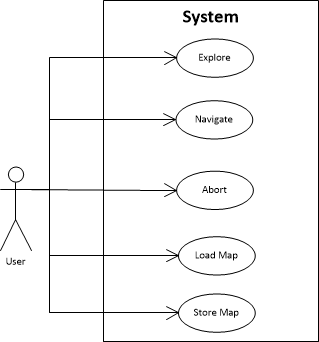
\includegraphics{img/usecases.png}
\caption{}
\label{fig:usecases}
\end{figure}

\subsection{Scenarios}
\labelssec{Scenarios}

\dots

\subsection{(Domain)model}

\textbf{CONSOLE MODEL}

\begin{lstlisting}

public interface IConsole {

public IMap explore(String EnvType, long maxMilsTime);	//modifier , primitive
public void navigate(double goalX, double goalY);		//modifier , primitive
public void navigate(double startX, double startY, double goalX, double goalY); //modifier , primitive
public void adbort();									//modifier , primitive

public void storeMap(IMap map, String filepath);		//modifier , primitive
public IMap loadMap(String filepath);					//modifier , primitive

public IMap getMap(); 									//property , primitive
public void getName();									//property , primitive

public String getDefaultRep();	// mapping , non-primitive
}

\end{lstlisting}

--- --- --- --- --- ---\\\\
\textbf{ROBOT MODEL}

\begin{lstlisting}
public interface IRobot {

public void move(String dir, double speed, double mils);//modifier , priitive
public void move(String dir, int steps);			//modifier , priitive
public void turn(double angle, double speed);		//modifier , priitive
public void stop();									//modifier , priitive

public void setMap(IMap map);						// property , primitive
public IMap getMap();								// property , primitive

public void navigateTo(double goalX, double goalY);	//modifier , priitive
public void navigate(double startX, double startY, double goalX, double goalY); 

public IMap explore(String EnvType, long maxMilsTime);//modifier , priitive

public String getName();							// property , primitive
public String getDefaultRep();						// mapping , non-primitive

}

\end{lstlisting}


\subsection{Test plan}
\dots
%===========================================================================
\section{Problem analysis}
\labelsec{ProblemAnalysis}
%===========================================================================

\textbf{Logic architecture}\\

Per soddisfare i requisiti del problema non � sufficiente utilizzare dei semplici componenti POJO, � necessario invece dotarsi di una architettura eterogenea e distribuita.\\


\textbf{Modello di Interazione}\\

Per quanto riguarda l'interazione, ho scelto un modello fortemente Event Driven. Gli eventi vengono emessi sia dalla Console che dal Robot, la netta distinzione in fasi di eleaborazione permette di sapere con certezza quali eventi possono essere generati in un determinato momento.\\

\textbf{Eventi e Contenuto Informativo}\\

Durante il normale funzionamento del sistema si verificano le seguenti interazioni:

\begin{itemize}
	\item \textbf{explore : explore( TYPE, MILS )} viene generato dalla Console quando l'utente decide di inziare l'Esplorazione dell'ambiente. Il payload indica il tipo di ambiente da esplorare (open / close) e il tempo massimo espresso in millisecondi;\\
	
	\item \textbf{navigate : navigate( GOAL )} oppure \textbf{navigate : navigate( START, GOAL )}, generato dalla Console quando l'utente decide di iniziare la navigazione, partendo da un mappa appena creata, oppure salvata precedentemente. Il payload indica la posizione GOAL e quella di START (opzionale) nel formato \textbf{position( X , Y )};\\
	
	\item \textbf{abort : abort}, generato dalla Console, indica che l'utente vuole terminare l'elaborazione in corso, che sia una Esplorazione oppure una Navigazione. Non sono necessari dati aggiuntivi;\\
	
	\item \textbf{end : end}, generato dal Robot, indica che ha terminato l'esecuzione dell'ultimo comando, che sia di Esplorazione o Navigazione. Non sono necessari dati aggiuntivi;\\
	
	\item \textbf{update : update( ELEMENT )}, generato dal Robot, comunica che � stata esplorata una nuova posizione della mappa che, di conseguenza, deve essere aggiornata. ELEMENT � uno dei seguenti:
	\begin{itemize}
		\item \textbf{obstacle( X, Y )};
		\item \textbf{clear( X , Y )};
		\item \textbf{border( X , Y )};
	\end{itemize}
\end{itemize}

\textbf{Comportamento delle Entit�}\\

\textbf{CONSOLE}

\begin{lstlisting}
RobotSystem exploreAndGo


/*
* ----------------------------------------------------
* EVENTS emitted by the system components
* ----------------------------------------------------
*/
// C to R, MILS is the maximum millisecond time
Event explore : explore(TYPE, MILS) 

// C to R
Event navigate : navigate(START, GOAL)

// C to R
Event navigate : navigate(GOAL) 

//C to R, abort exploration or navigation
Event abort : abort 

//R to C, termination of exploration or navigation
Event end : end 

//R to C, update the Map
Event update : update(ELEMENT)

/*
* EVENTS FROM THE GUI
*/
Event local_gui_command : command(C)


/*
* ----------------------------------------------------
* CONTEXT for the Robot as independent device (standdalone)
* ----------------------------------------------------
*/
Context ctxRobot ip [ host="localhost" port=8020] -standalone 

/*
* ----------------------------------------------------
* CONTEXT for the Console
* ----------------------------------------------------
*/ 
Context ctxConsole ip [ host="localhost" port=8010]


/*
* ----------------------------------------------------
* CONSOLE with custom GUI
* ----------------------------------------------------
*/

QActor console context ctxConsole -g cyan{



Plan init normal
println(console(start));
switchToPlan waitCommand

//---------------------------------------------------------------------------

Plan waitCommand

println("Wait for user command");

sense time(999999999) local_gui_command -> continue;
[ ?? tout(X,Y) ] switchToPlan handleTimeout;
memoCurrentEvent;
printCurrentEvent;

onEvent local_gui_command : command(explore(TYPE, MILS))
				 ->	switchToPlan exploration;
				 
[ !? have_map ] onEvent local_gui_command : command(navigate(START, GOAL))
				 -> switchToPlan navigation;
				 
[ !? have_map ] onEvent local_gui_command : command(navigate(GOAL))
				 -> switchToPlan navigation;
				 
onEvent local_gui_command : command(load(PATH))
				 -> switchToPlan loadMap;

repeatPlan 0

//---------------------------------------------------------------------------

Plan exploration

println("EXPLORE");

// discard all old map data

[?? msg(local_gui_command, "event", SENDER,
				 none, command(explore(TYPE, MILS)), MSGNUM)]
				 emit explore : explore(TYPE, MILS);

sense time(999999999) update, local_gui_command, end
				 -> continue, continue, continue;
				 
[ ?? tout(X,Y) ] switchToPlan handleTimeout;
memoCurrentEvent;
printCurrentEvent;

onEvent update : update(ELEMENT)
				 -> switchToPlan updateMap;
				 
onEvent local_gui_command : command(abort)
				 -> switchToPlan abortLastCommand;
				 
onEvent end : end
				 -> switchToPlan endOfExploration;

repeatPlan 0

//---------------------------------------------------------------------------

Plan endOfExploration
println("do you want to save the map or explore again??");

sense time(999999999) local_gui_command -> continue;
[ ?? tout(X,Y) ] switchToPlan handleTimeout;
memoCurrentEvent;
printCurrentEvent; 	

onEvent local_gui_command : command(store(PATH))
				 -> switchToPlan storeMap;
				 
onEvent local_gui_command : command(explore(TYPE, MILS))
				 ->	switchToPlan exploration

//---------------------------------------------------------------------------

Plan updateMap resumeLastPlan
[?? msg(update, "event", SENDER, none, update(ELEMENT), MSGNUM)] println(update(ELEMENT))

//---------------------------------------------------------------------------

Plan navigation resumeLastPlan
println("NAVIGATE");

//---------------------------------------------------------------------------

[?? msg(local_gui_command, "event", SENDER, none,
				 command(navigate(START, GOAL)), MSGNUM)]
				 emit navigate : navigate(START, GOAL);
				 
[?? msg(local_gui_command, "event", SENDER, none,
				 command(navigate(GOAL)), MSGNUM)]
				 emit navigate : navigate(GOAL);

sense time(999999999) local_gui_command, end
				 -> continue, continue;
				 
[ ?? tout(X,Y) ] switchToPlan handleTimeout;
memoCurrentEvent;
printCurrentEvent;

onEvent local_gui_command : command(abort)
				 -> switchToPlan abortLastCommand;
				 
onEvent end : end
				 -> switchToPlan endOfNavigation

//---------------------------------------------------------------------------

Plan endOfNavigation
println("Robot reached the GOAL position");
switchToPlan waitCommand 	

//---------------------------------------------------------------------------

Plan loadMap resumeLastPlan
println("Map loaded");
[?? msg(local_gui_command, "event", SENDER, none,
				 command(load(PATH)), MSGNUM)]
				 addRule have_map
				 
// <-- waitCommand

//---------------------------------------------------------------------------

Plan storeMap 
println("Map saved");
[?? msg(local_gui_command, "event", SENDER, none,
				 command(store(PATH)), MSGNUM)]
				 addRule have_map;
				 
switchToPlan waitCommand

//---------------------------------------------------------------------------

Plan abortLastCommand
println("Abort");
emit abort : abort;
switchToPlan waitCommand



Plan handleTimeout
println("timeout!! GOODBYE")

}


Robot scout QActor robot context ctxRobot{
Plan init normal
println( "NEVER HERE. I'm just a place holder" ) 
}

\end{lstlisting}

� molto chiara la distinzione in fasi di elaborazione, � infatti possibile rappresentare il comportamento della Console, e dell'intero sistema come una macchina a stati finiti.

Le fasi principali sono Exploration e Navigation, troviamo inoltre le fasi di LoadMap, StoreMap e UpdateMap.
Infine sono presenti numerose fasi che aiutano a rendere pi� semplice e funzionale l'elaborazione.

\subsection{Abstraction gap}

\dots

\subsection{Risk analysis}

\dots
%===========================================================================
\section{Work plan}
\labelsec{wplan}
%===========================================================================

\begin{itemize}
	\item[\checkmark] Definizione dei requisiti
	\item[\checkmark] Analisi del Problema
	\item[\checkmark] modello per la Console (linguaggio naturale)
	\item[\checkmark] modello per il Robot (linguaggio naturale)
	\item[\checkmark] modello per la Console in maniera formale
	\item modello per il Robot in maniera formale
	\item Esplorazione "close" con confini definiti
	\item Ricerca dei confini "close"
	\item Esplorazione "open"
	\item Navigazione
\end{itemize}

%===========================================================================
\section{Project}
\labelsec{Project}
%===========================================================================

\subsection{Structure}
\subsection{Interaction}
\subsection{Behavior}

%===========================================================================
\section{Implementation}
\labelsec{Implementation}
%===========================================================================

%===========================================================================
\section{Testing}
\labelsec{testing}
%===========================================================================

%===========================================================================
\section{Deployment}
\labelsec{Deployment}
%===========================================================================

%===========================================================================
\section{Maintenance}
\labelsec{Maintenance}
%===========================================================================
\newpage
See \cite{natMol09} until page 11 (\texttt{CMM}) and pages 96-105.

%===========================================================================
\section{Information about the author}
\labelsec{Author}
%===========================================================================

\vskip.5cm
%%% \begin{figure}
\begin{tabular}{ | c |  }
\hline
  % after \\: \hline or \cline{col1-col2} \cline{col3-col4} ...
  Photo of the author 
  \\
\hline
   
\includegraphics[scale = 0.3]{img/me.jpg}
  \\
\hline
\end{tabular}


%%% \begin{itemize}
%%% \item Titolo di studio:\\ \\
%%% \item Interessi particolari:\\ \\
%%% \item Ha sostenuto fino ad oggi il seguente numero di esami:\\ \\
%%% \item Deve ancora sostenere i seguenti esami del I anno:\\ \\
%%% \item Prevede di svolgere un tirocinio presso:\\ \\
%%% \item Prevede di laurearsi nella sessione:\\ \\
%%% \item Intende proseguire gli studi per conseguire: \\  \\  \\
%%%   	presso la sede universitaria di: \\ \\
%%% \item Intende entrare subito nel mondo del lavoro presso : \\ \\
%%% \end{itemize}

 
\appendix


\bibliographystyle{abbrv}
\bibliography{biblio}

\end{document}












